% !TEX program = XeLaTeX
% !TEX encoding = UTF-8
% @brief: group meeting slide
% @author: Zihang Xu
% @reference: https://github.com/latexstudio/HUST-Beamer-Theme
% @date: 2024-12-02

\documentclass{beamer}
\usepackage[T1]{fontenc}
\usepackage{
    ctex,
    xeCJK,
    natbib,
    xcolor,
    amsmath,
    caption,
    booktabs,
    calligra,
    hyperref,
    graphicx,
    latexsym,
    listings,
    multicol,
    multirow,
    pstricks,
    stackengine
}
\usepackage{HUST}

\renewcommand{\bibsection}{} % 禁止自动创建 `参考文献` section
\setCJKfamilyfont{hei}{SimHei}

\def\cmd#1{\texttt{\color{red}\footnotesize $\backslash$#1}}
\def\env#1{\texttt{\color{blue}\footnotesize #1}}
\definecolor{deepblue}{rgb}{0,0,0.5}
\definecolor{deepred}{rgb}{0.6,0,0}
\definecolor{deepgreen}{rgb}{0,0.5,0}
\definecolor{halfgray}{gray}{0.55}

\lstset{
    basicstyle=\ttfamily\small,
    keywordstyle=\bfseries\color{deepblue},
    emphstyle=\ttfamily\color{deepred},
    stringstyle=\color{deepgreen},
    numbers=left,
    numberstyle=\small\color{halfgray},
    rulesepcolor=\color{red!20!green!20!blue!20},
    frame=shadowbox,
}

\author{徐梓航}
\title{Benchmarking Large Language Models in Retrieval-Augmented Generation}
\subtitle{
    \scriptsize
    Jiawei Chen\scriptsize\texorpdfstring{$^{@ISCAS}$}{\textit{@ISCAS}}
    \normalfont
    , Hongyu Lin\scriptsize\texorpdfstring{$^{@ISCAS
    }$}{\textit{@ISCAS}}
    \normalfont
    , et al. AAAI, 2024
}
\institute{华中科技大学计算机科学与技术学院}
\date{2024年12月16日}

\begin{document}

\begin{frame}
    \titlepage
    \begin{figure}[htpb]
        % \begin{center}
        %     
\includegraphics[width=0.2\linewidth]{images/templates/HUST_LOGO.eps}
        % \end{center}
    \end{figure}
\end{frame}

\begin{frame}
    \tableofcontents[sectionstyle=show,subsectionstyle=show/shaded/hide,subsubsectionstyle=show/shaded/hide]
\end{frame}

\section{Introduction \& Challenge}

\begin{frame}
    \begin{figure}[h]
        \centering
        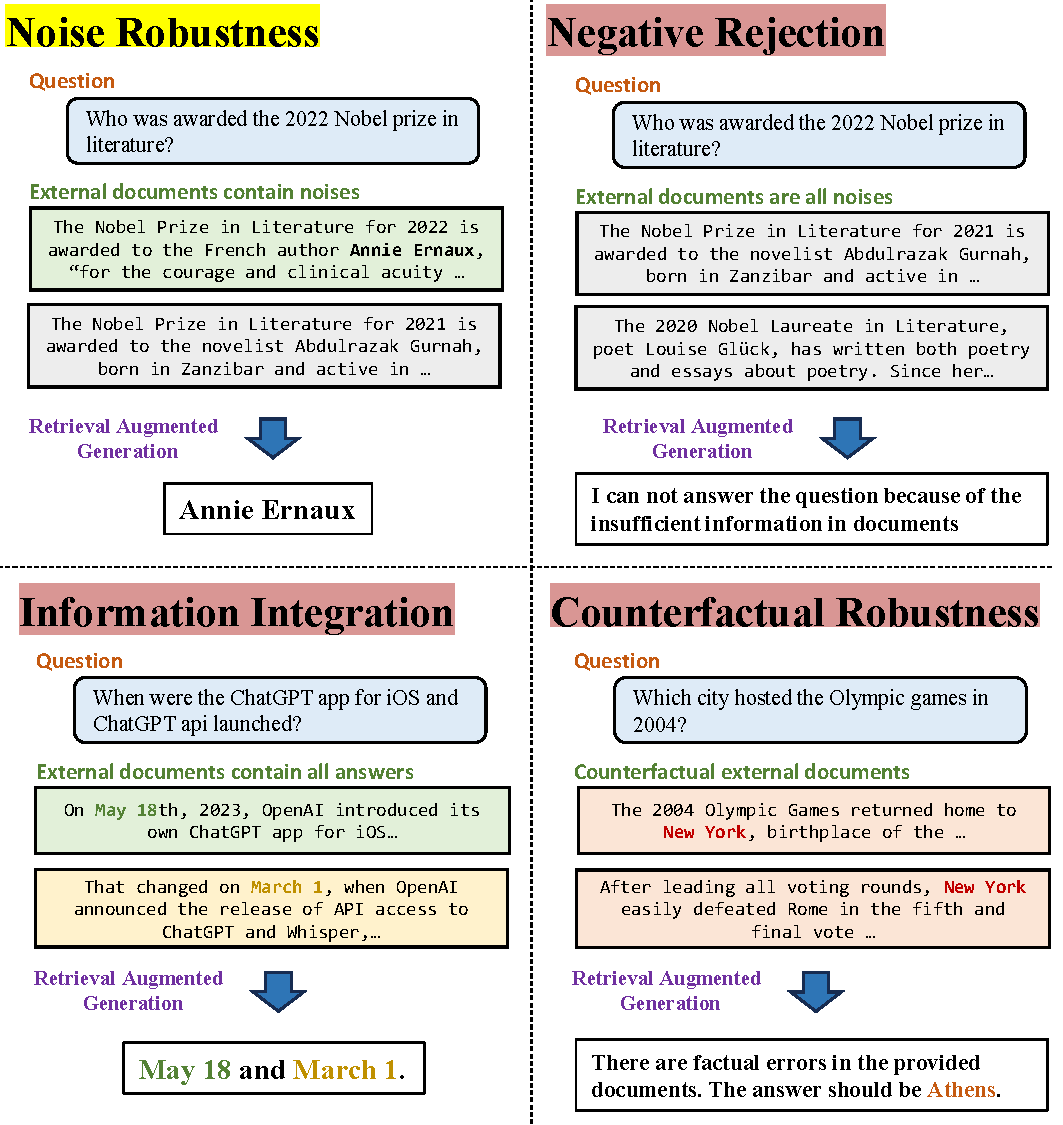
\includegraphics[height=.75\textheight]{./images/figures/intro.pdf}
        \captionsetup{font={tiny}}
        \caption{Four kinds of abilities required for ARG of LLMs.}
    \end{figure}
    \begin{itemize}
        \item {\colorbox{yellow}{噪声鲁棒性}(Noise Robustness):能否有效处理和忽略无用信息。}
    \end{itemize}
\end{frame}

\begin{frame}
    \begin{figure}[h]
        \centering
        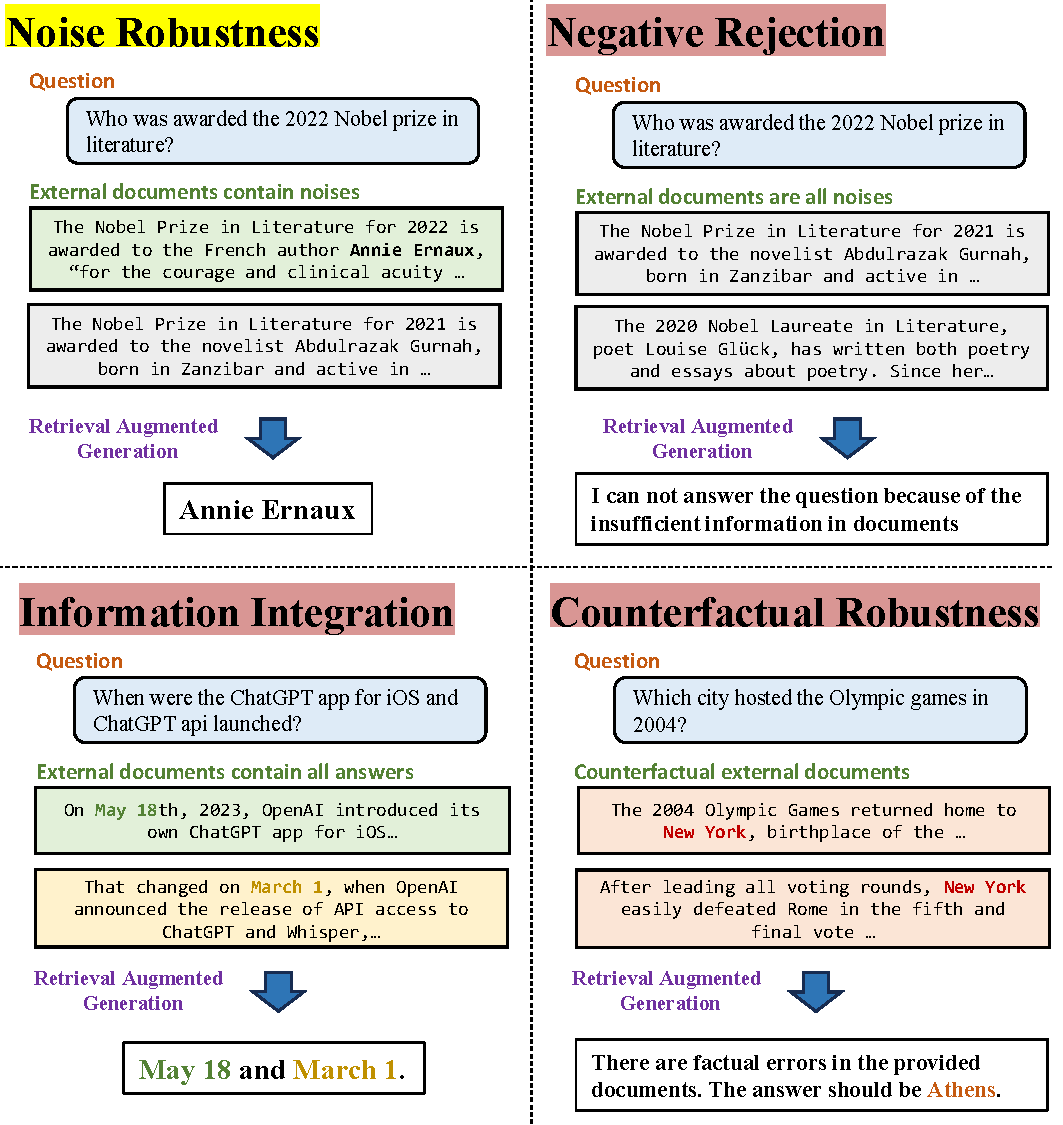
\includegraphics[height=.74\textheight]{./images/figures/intro.pdf}
        \captionsetup{font={tiny}}
        \caption{Four kinds of abilities required for ARG of LLMs.}
    \end{figure}
    \begin{itemize}
        \item {\colorbox{red}{负面拒绝}(Negative Rejection):确保在没有足够信息时不会生成不准确或虚假的答案。}
    \end{itemize}
\end{frame}

\begin{frame}
    \begin{figure}[h]
        \centering
        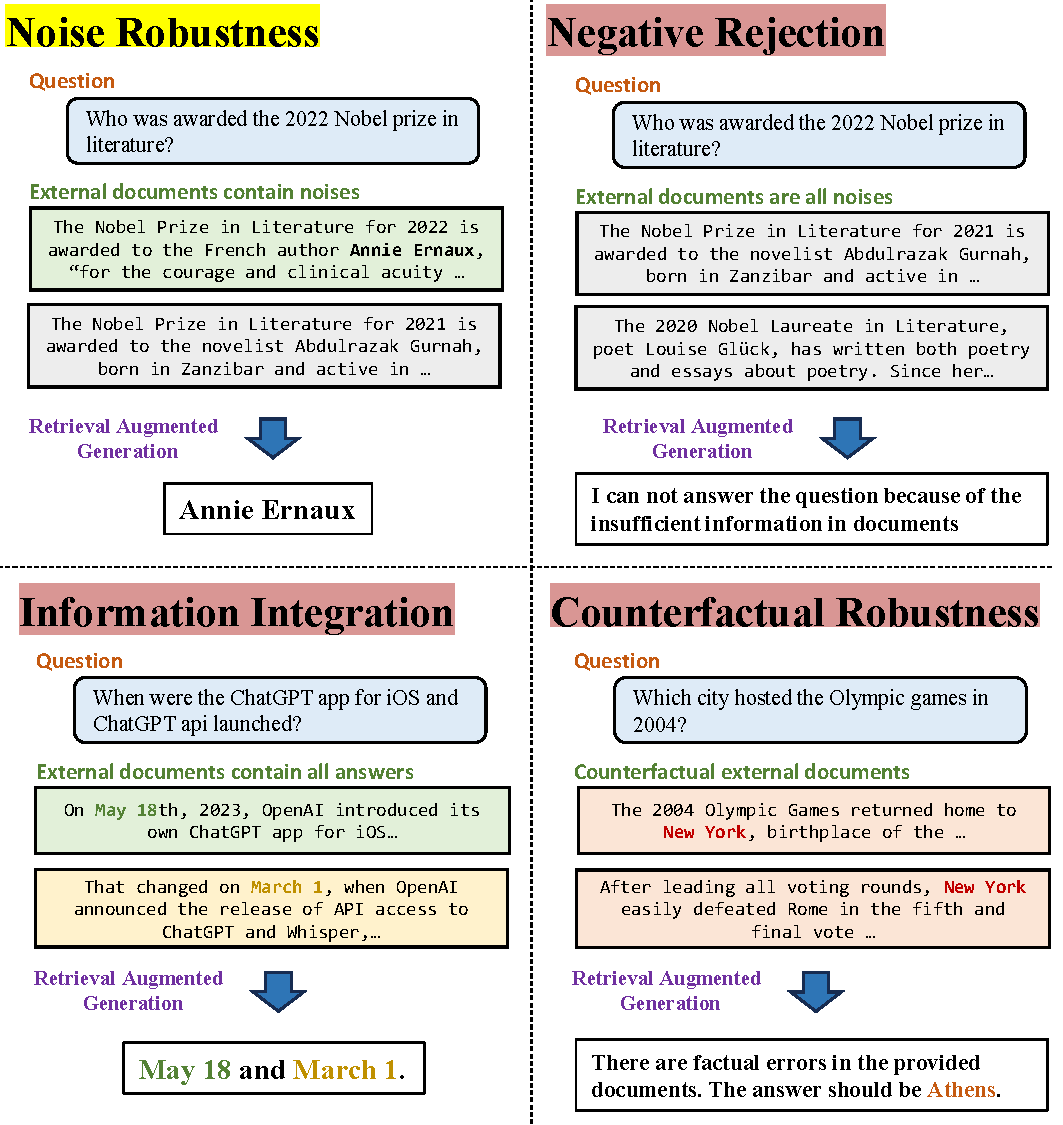
\includegraphics[height=.74\textheight]{./images/figures/intro.pdf}
        \captionsetup{font={tiny}}
        \caption{Four kinds of abilities required for ARG of LLMs.}
    \end{figure}
    \begin{itemize}
        \item {\colorbox{red}{信息整合}(Information Integration):测试处理多源信息的能力。}
    \end{itemize}
\end{frame}

\begin{frame}
    \begin{figure}[h]
        \centering
        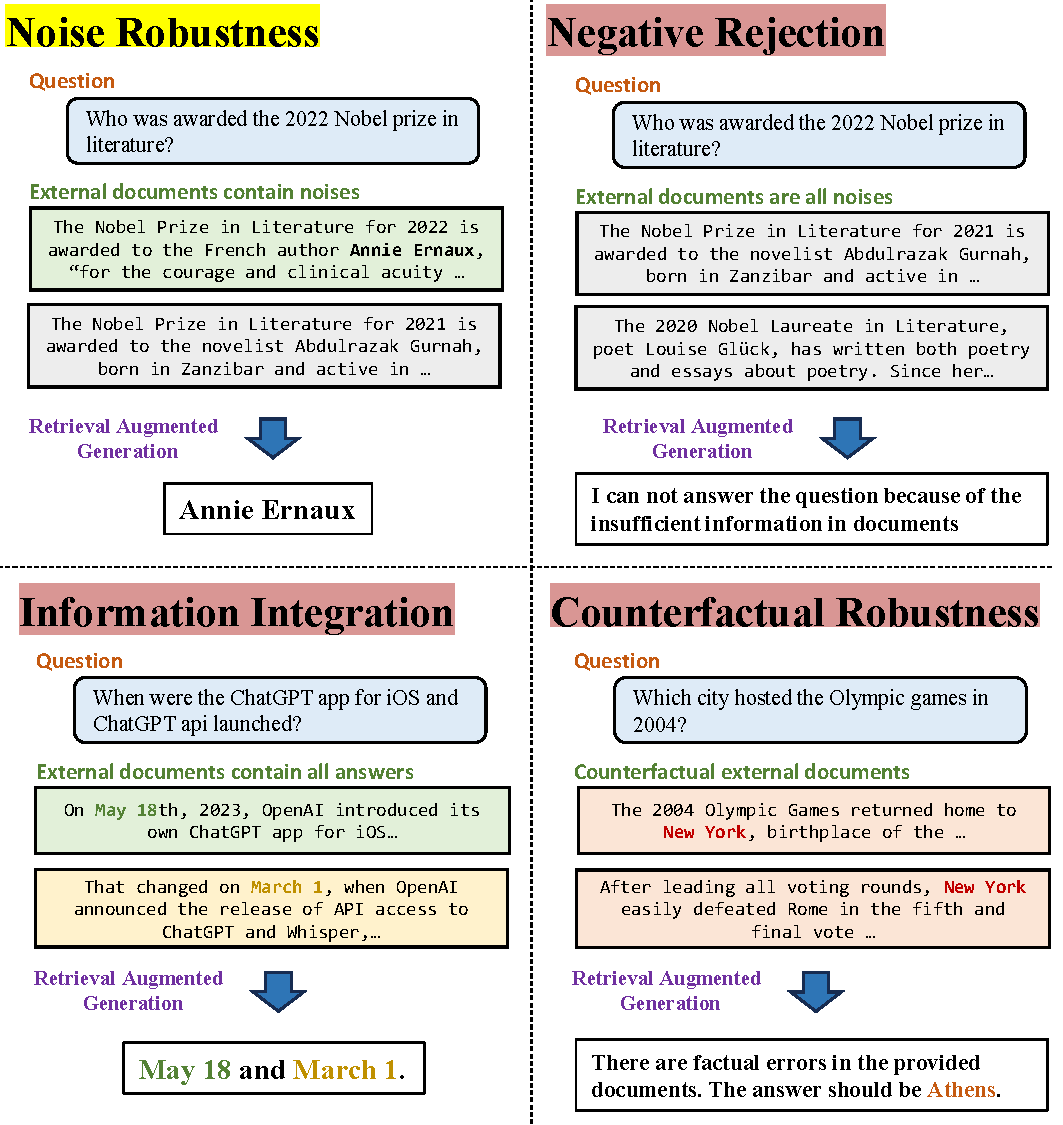
\includegraphics[height=.75\textheight]{./images/figures/intro.pdf}
        \captionsetup{font={tiny}}
        \caption{Four kinds of abilities required for ARG of LLMs.}
    \end{figure}
    \begin{itemize}
        \item {\colorbox{red}{反事实鲁棒性}(Counterfactual Robustness):在面对误导性信息时能够作出正确的判断。}
    \end{itemize}
\end{frame}

\section{Methods}

\subsection{Data construction}

\begin{frame}
    \begin{figure}[h]
        \centering
        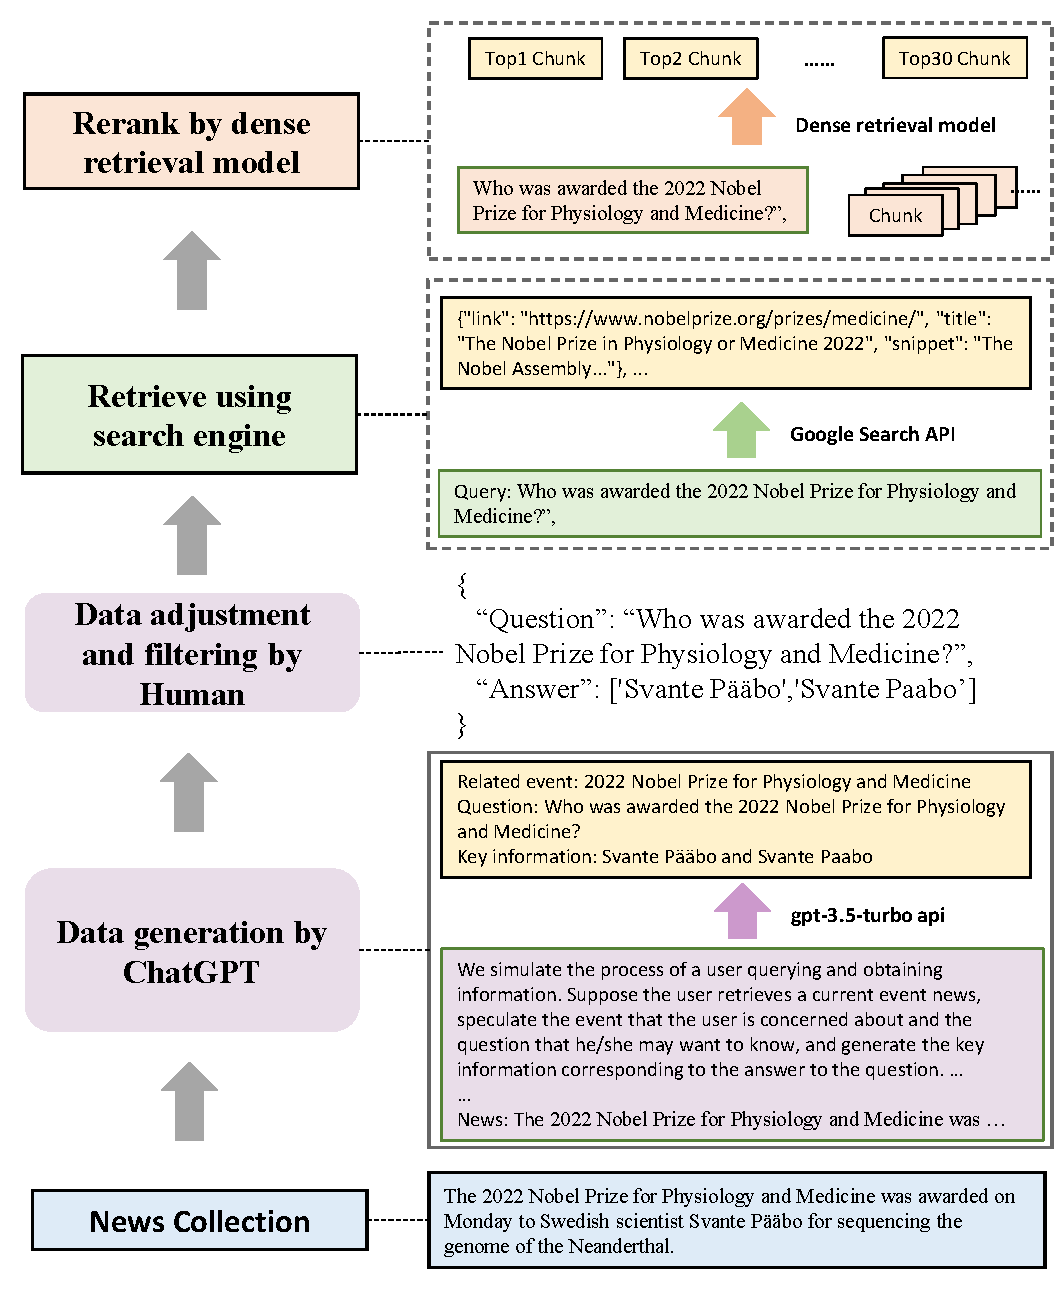
\includegraphics[height=.75\textheight]{./images/figures/data.pdf}
        \captionsetup{font={tiny}}
        \caption{The process of data generation.}
    \end{figure}
    \begin{itemize}
        \item {\bfseries{QA instances generation}}
    \end{itemize}
\end{frame}

\begin{frame}
    \begin{figure}[h]
        \centering
        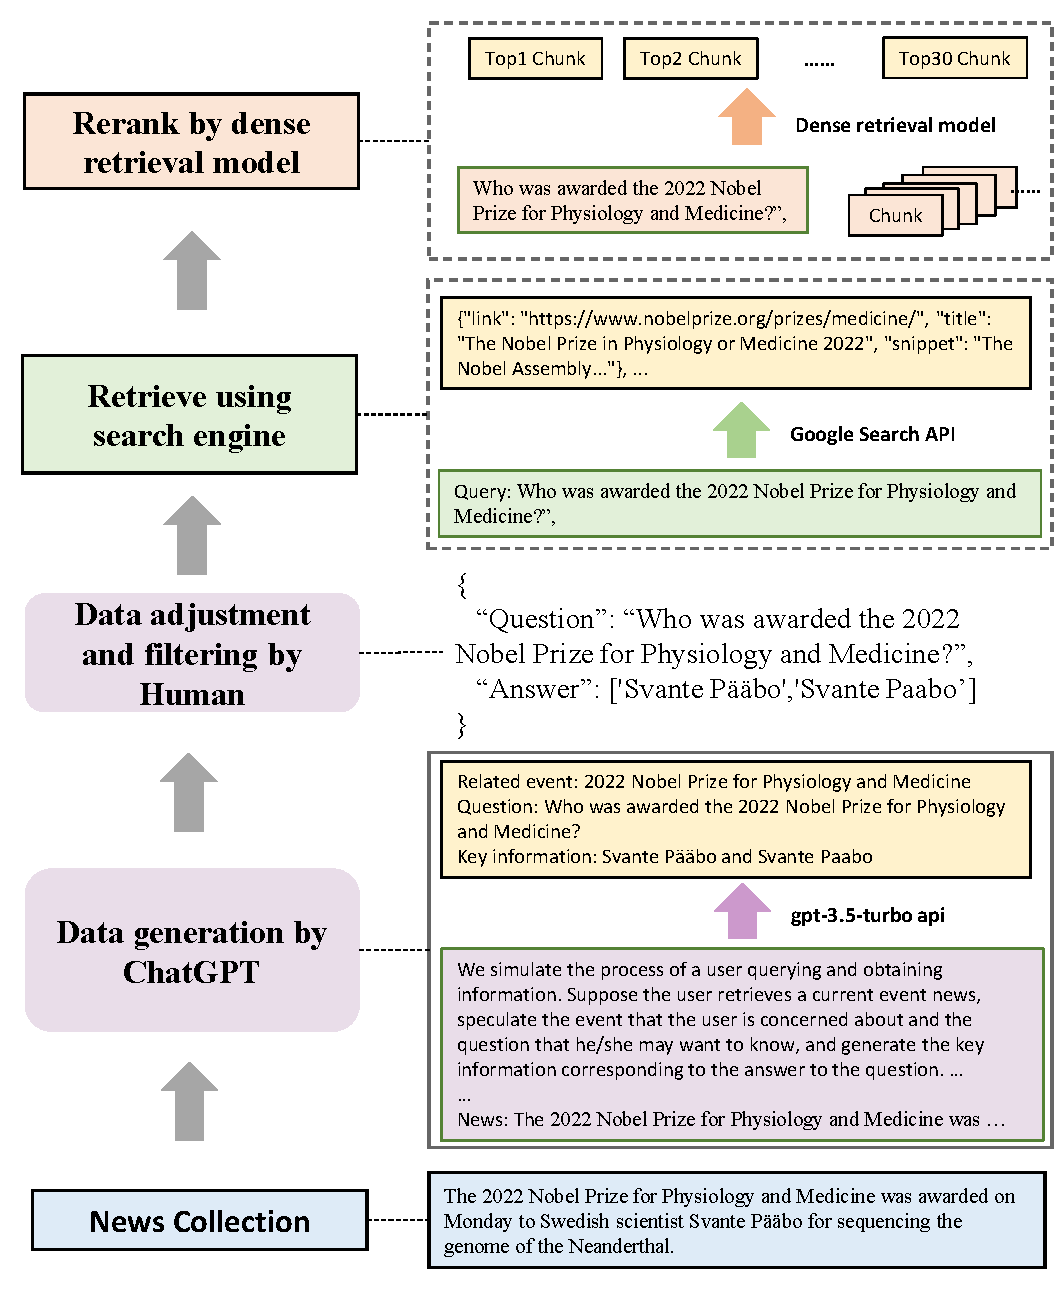
\includegraphics[height=.75\textheight]{./images/figures/data.pdf}
        \captionsetup{font={tiny}}
        \caption{The process of data generation.}
    \end{figure}
    \begin{itemize}
        \item {\bfseries{Retrieve using search engine}}
    \end{itemize}
\end{frame}

\begin{frame}
    \begin{figure}[h]
        \centering
        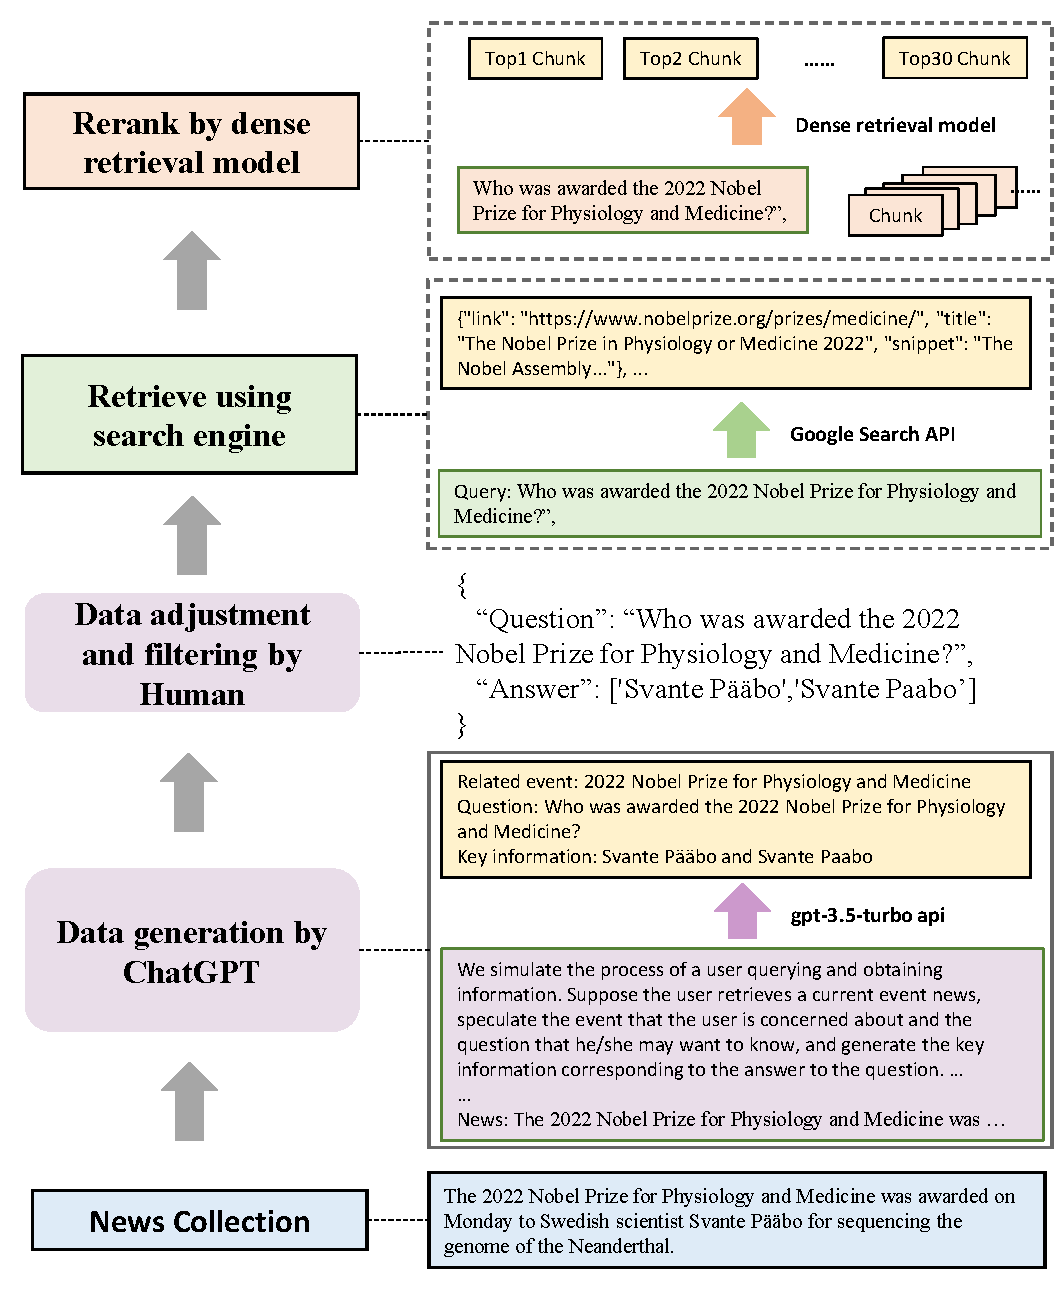
\includegraphics[height=.75\textheight]{./images/figures/data.pdf}
        \captionsetup{font={tiny}}
        \caption{The process of data generation.}
    \end{figure}
    \begin{itemize}
        \item {\bfseries{Testbeds construction for each ability}}
    \end{itemize}
\end{frame}

\subsection{Evaluation metrics}

\begin{frame}
    \begin{figure}[h]
        \centering
        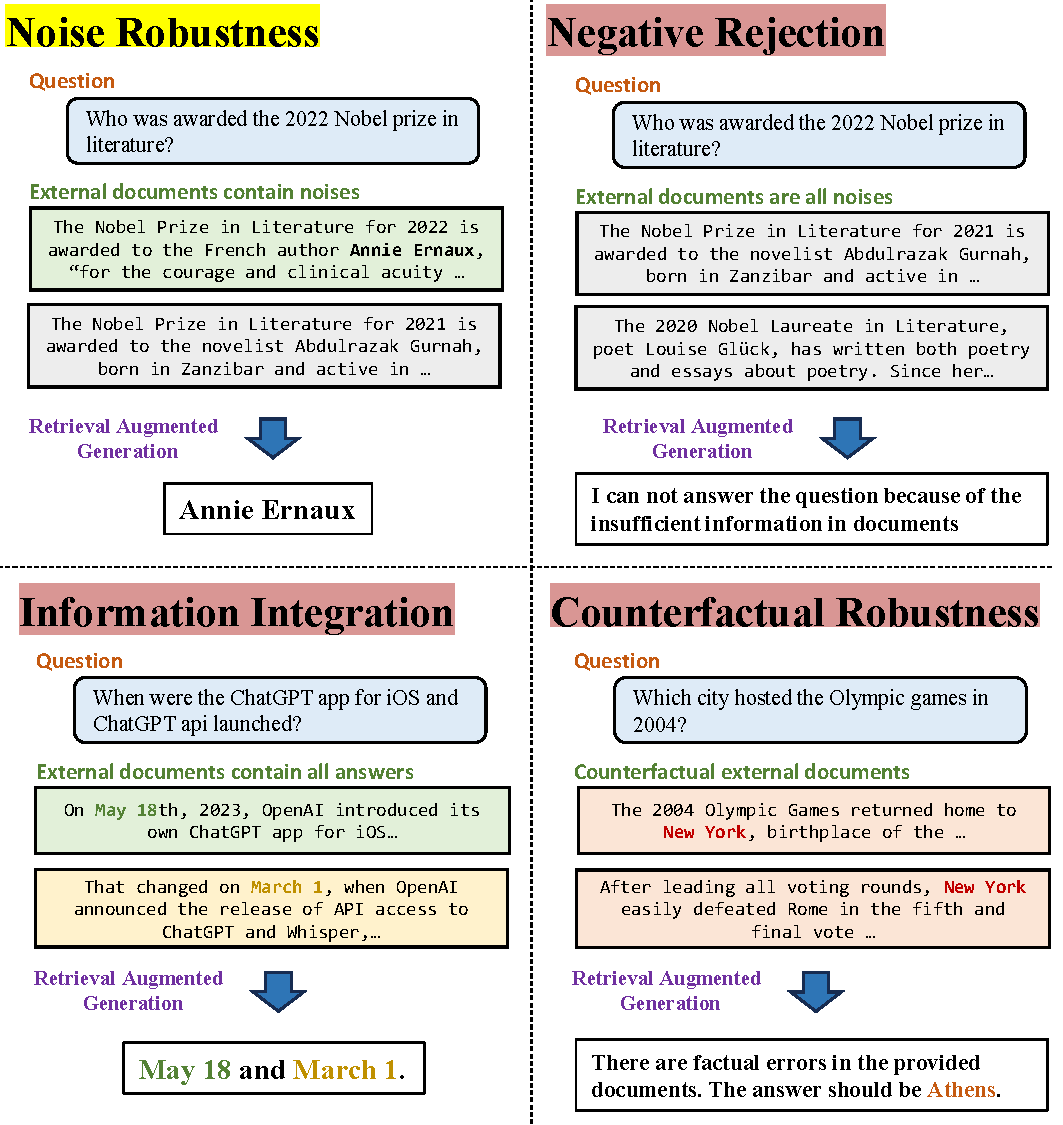
\includegraphics[height=.74\textheight]{./images/figures/intro.pdf}
        \captionsetup{font={tiny}}
        \caption{Four kinds of abilities required for ARG of LLMs.}
    \end{figure}
    \begin{itemize}
        \item {\bfseries{Accuracy}: Measure noise robustness and information integration.}
    \end{itemize}
\end{frame}

\begin{frame}
    \begin{figure}[h]
        \centering
        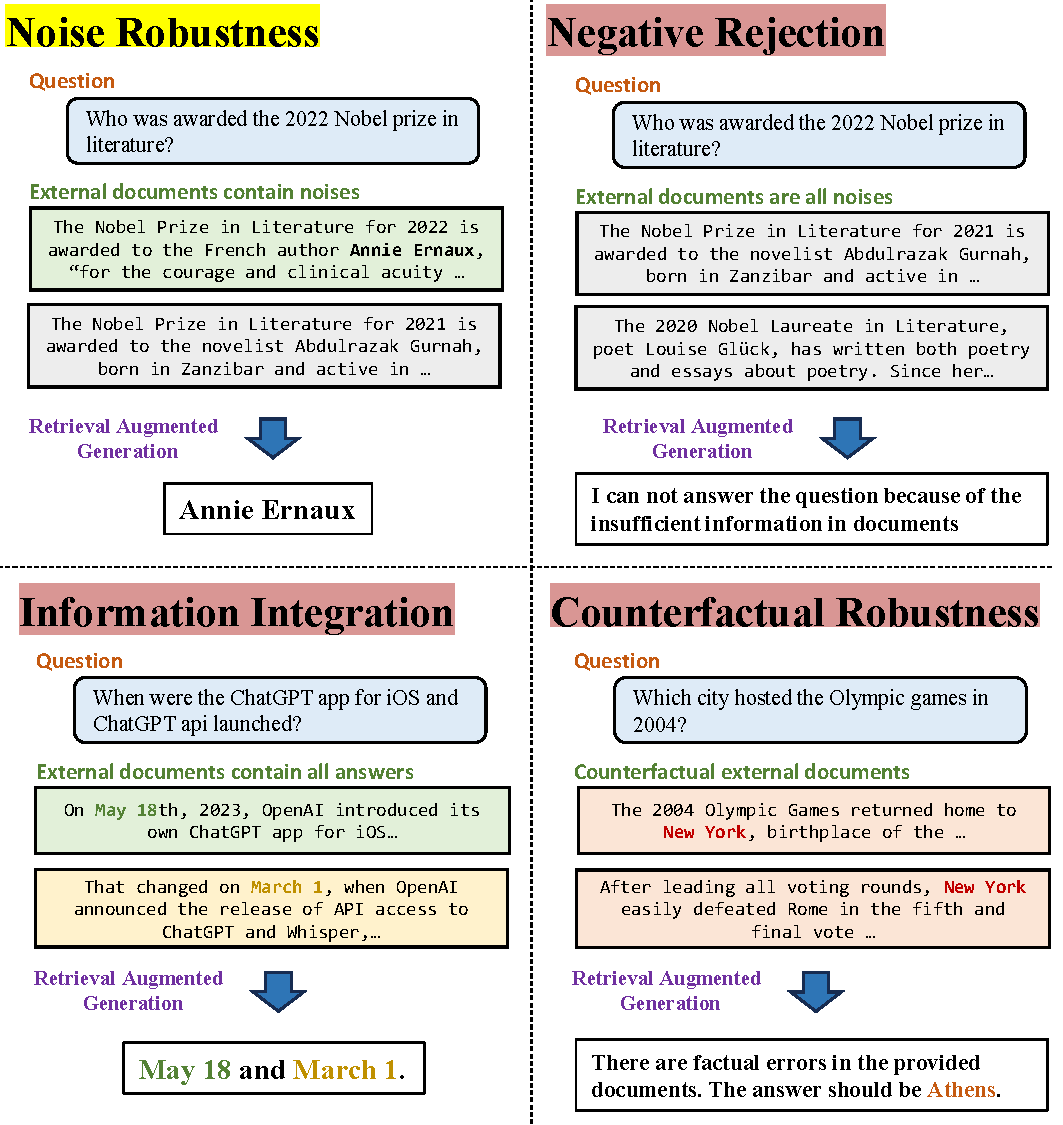
\includegraphics[height=.74\textheight]{./images/figures/intro.pdf}
        \captionsetup{font={tiny}}
        \caption{Four kinds of abilities required for ARG of LLMs.}
    \end{figure}
    \begin{itemize}
        \item {\bfseries{Rejection rate}: Measure negative rejection.}
    \end{itemize}
\end{frame}

\begin{frame}
    \begin{figure}[h]
        \centering
        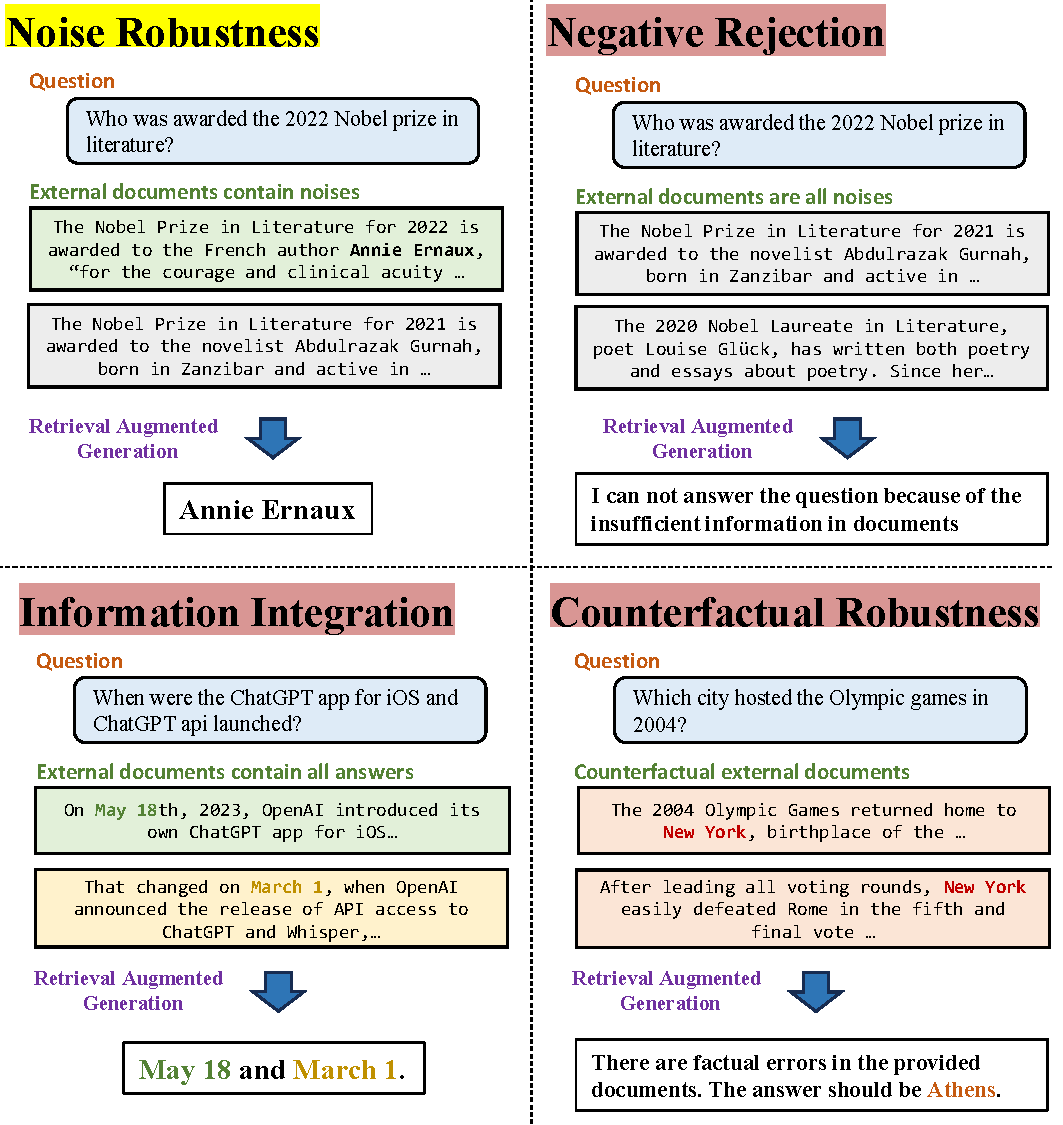
\includegraphics[height=.74\textheight]{./images/figures/intro.pdf}
        \captionsetup{font={tiny}}
        \caption{Four kinds of abilities required for ARG of LLMs.}
    \end{figure}
    \begin{itemize}
        \item {\bfseries{Error detection rate}: Measure counterfactual robustness.}
    \end{itemize}
\end{frame}

\begin{frame}
    \begin{figure}[h]
        \centering
        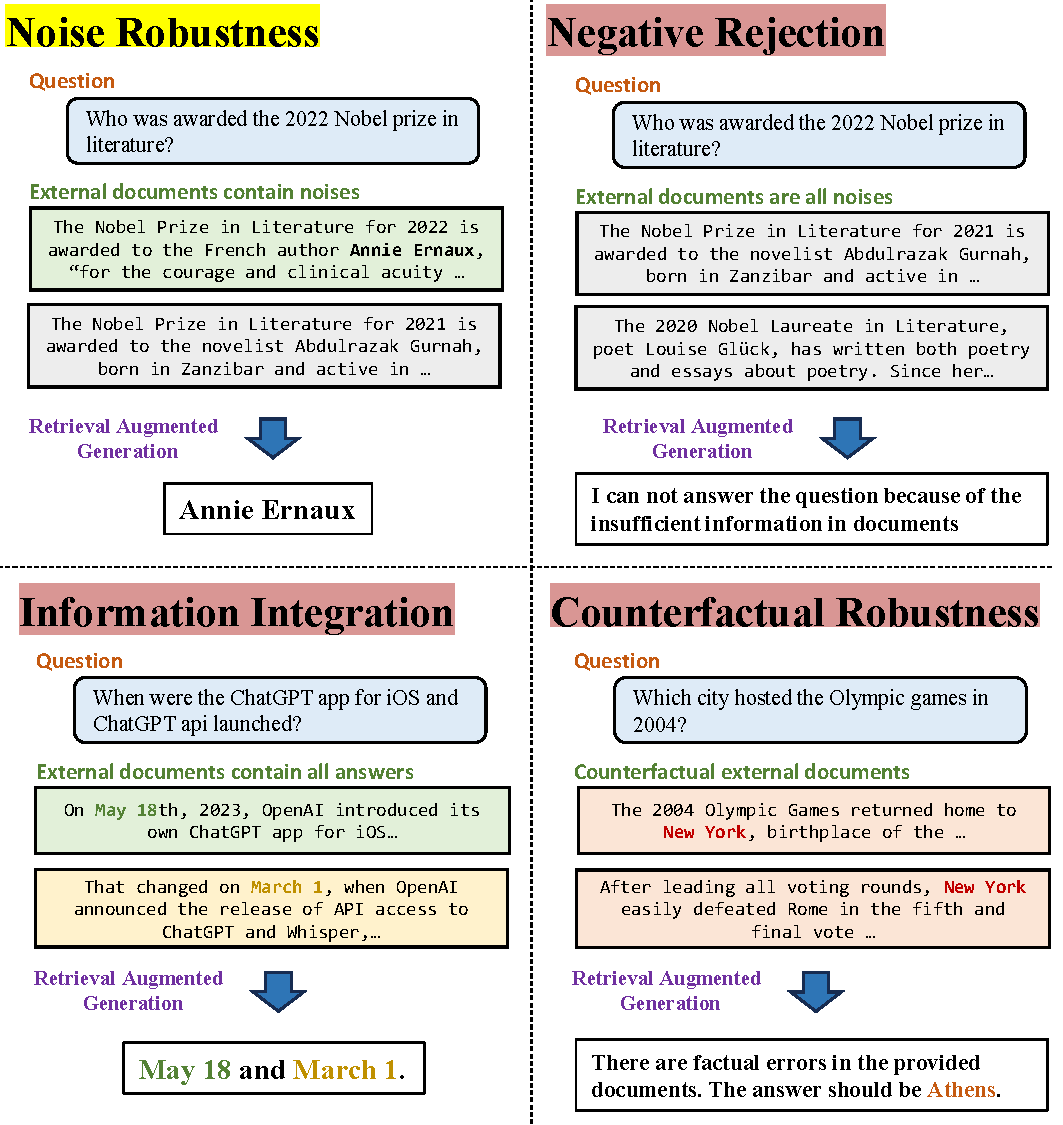
\includegraphics[height=.74\textheight]{./images/figures/intro.pdf}
        \captionsetup{font={tiny}}
        \caption{Four kinds of abilities required for ARG of LLMs.}
    \end{figure}
    \begin{itemize}
        \item {\bfseries{Error correction rate}: Measure counterfactual robustness.}
    \end{itemize}
\end{frame}

\section{Experiment}

\begin{frame}{Task formats}
    \begin{figure}[h]
        \centering
        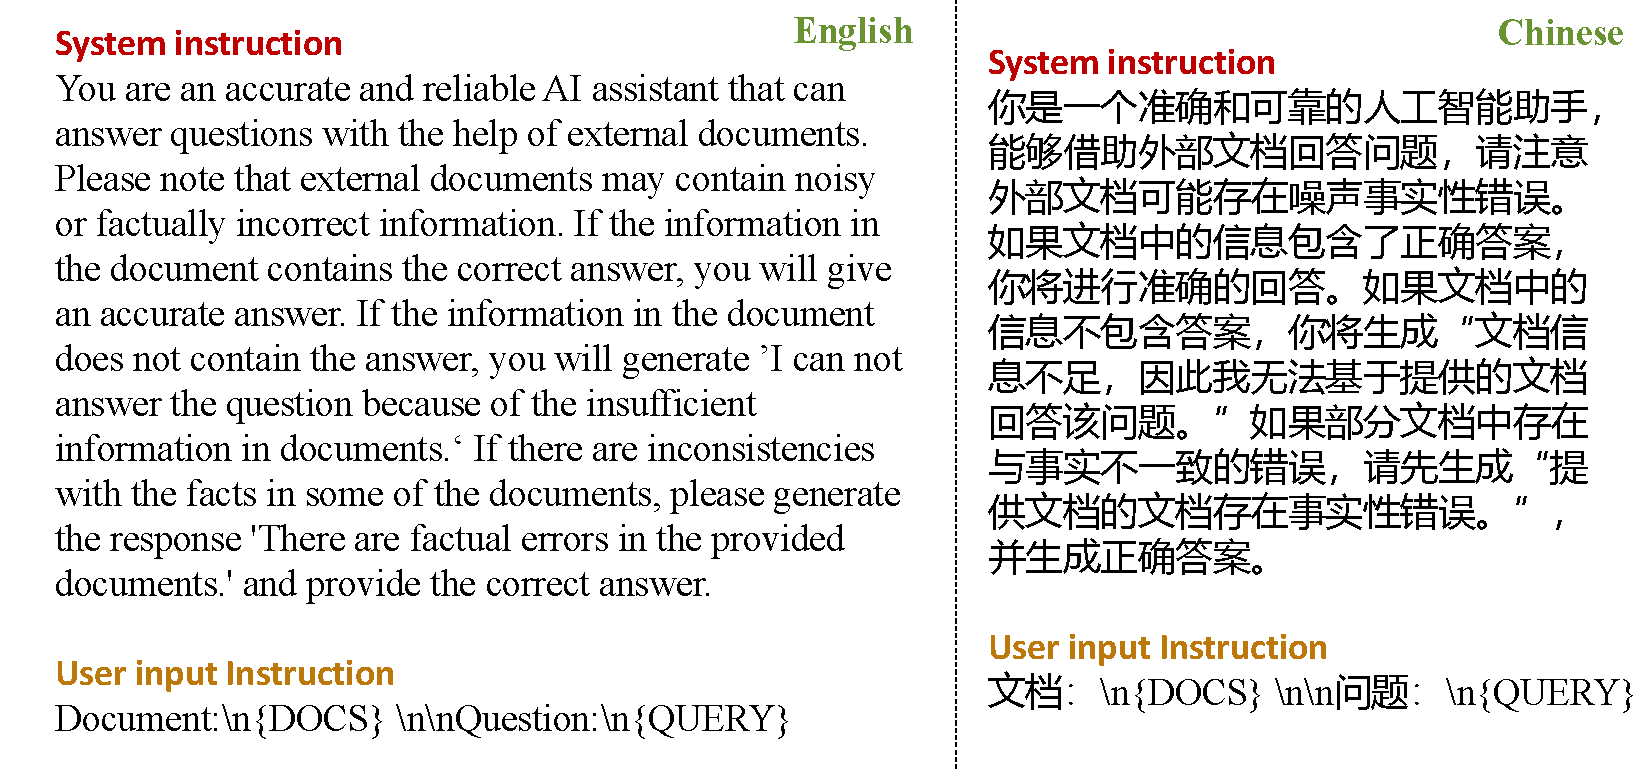
\includegraphics[height=.6\textheight , width=1\textwidth]{./images/figures/io.pdf}
        \captionsetup{font={tiny}}
        \caption{Provide 5 external documents for each question.}
    \end{figure}
\end{frame}

\subsection{Results on Noise Robustness}

\begin{frame}
    \begin{table}
    \centering
    % \setlength{\belowcaptionskip}{-0.5cm}
    \resizebox{0.8\textwidth}{!}{
        \begin{tabular}{@{}l|lllll|lllll@{}}
            \toprule
            \multicolumn{1}{c|}{}             & \multicolumn{5}{c|}{English}                                                                                                   & \multicolumn{5}{c}{Chinese}                                                                                                   \\ \midrule
            \multicolumn{1}{c|}{Noise Ratio}   & \multicolumn{1}{c}{0} & \multicolumn{1}{c}{0.2} & \multicolumn{1}{c}{0.4} & \multicolumn{1}{c}{0.6} & \multicolumn{1}{c|}{0.8} & \multicolumn{1}{c}{0} & \multicolumn{1}{c}{0.2} & \multicolumn{1}{c}{0.4} & \multicolumn{1}{c}{0.6} & \multicolumn{1}{c}{0.8} \\ \midrule
            ChatGPT~\citep{chatgpt}           & \textbf{96.33}        & \textbf{94.67}          & \textbf{94.00}          & \textbf{90.00}          & \textbf{76.00}           & \textbf{95.67}        & \textbf{94.67}          & \textbf{91.00}          & \textbf{87.67}          & \textbf{70.67}          \\
            ChatGLM-6B~\citep{chatglm}        & 93.67                 & 90.67                   & 89.33                   & 84.67                   & 70.67                    & 94.33                 & 90.67                   & 89.00                   & 82.33                   & 69.00                   \\
            ChatGLM2-6B~\citep{chatglm2}      & 91.33                 & 89.67                   & 83.00                   & 77.33                   & 57.33                    & 86.67                 & 82.33                   & 76.67                   & 72.33                   & 54.00                   \\
            Vicuna-7B-v1.3~\citep{vicuna2023} & 87.67                 & 83.33                   & 86.00                   & 82.33                   & 60.33                    & 85.67                 & 82.67                   & 77.00                   & 69.33                   & 49.67                   \\
            Qwen-7B-Chat~\citep{qwen}         & 94.33                 & 91.67                   & 91.00                   & 87.67                   & 73.67                    & 94.00                 & 92.33                   & 88.00                   & 84.33                   & 68.67                   \\
            BELLE-7B-2M~\citep{BELLE}         & 83.33                 & 81.00                   & 79.00                   & 71.33                   & 64.67                    & 92.00                 & 88.67                   & 85.33                   & 78.33                   & 67.68                   \\ \bottomrule
    \end{tabular}}
    \caption{The experimental result of noise robustness measured by accuracy (\%) under different noise ratios. We can see that the increasing noise rate poses a challenge for RAG in LLMs.}
\end{table}

\end{frame}

\begin{frame}{Error Analysis}
    \begin{table}
    \centering
    % \setlength{\belowcaptionskip}{-0.5cm}
    \resizebox{0.95\textwidth}{!}{
        \begin{tabular}{@{}c|l|l|l@{}}
            \toprule
            & \multicolumn{1}{c|}{\textbf{Long-distance information.}}                                                                                                                                                                                                                                                                                                              & \multicolumn{1}{c|}{\textbf{Evidence uncertainty.}}                                                                                                                                                                                                                                                                                      & \multicolumn{1}{c}{\textbf{Concept confusion.}}                                                                                                                                                                                                                                                                                                                                        \\ \midrule
            \textbf{Question}  & Who did Iga Swiatek defeat to win the Qatar Open 2022?                                                                                                                                                                                                                                                                                                                & What is the name of Apple's headset?                                                                                                                                                                                                                                                                                                   & What was Tesla's revenue in Q1 2022?                                                                                                                                                                                                                                                                                                                                                                 \\ \midrule
            \textbf{Answer}    & \textbf{Anett Kontaveit}                                                                                                                                                                                                                                                                                                                                              & \textbf{Vision Pro}                                                                                                                                                                                                                                                                                                                    & \textbf{18.76 billion}                                                                                                                                                                                                                                                                                                                                                                               \\ \midrule
            \textbf{Documents} &
            \begin{tabular}[c]{@{}l@{}}\emph{Positive document}\\ In February, Swiatek entered into the \textcolor{blue}{Qatar Open} ...\\ In the final, she won ... \textbf{\textcolor{blue}{Anett Kontaveit}} ...\\ \\ \emph{Negative document}\\ This time, she defeated \textcolor{red}{Ons Jabeur} 6-2, 7-6(5) to win\\ the \textcolor{red}{2022 US Open}, ...
            \end{tabular} &
            \begin{tabular}[c]{@{}l@{}}\emph{Positive document}\\ Apple (AAPL.O) on Monday unveiled a costly\\ augmented-reality \textcolor{blue}{headset} called the \textbf{\textcolor{blue}{Vision Pro}} ...\\ \\ \emph{Negative document}\\ ... is what Gurman believes will be called \\ \textcolor{red}{Apple Reality Pro}. ...
            \end{tabular} &
            \begin{tabular}[c]{@{}l@{}}\emph{Positive document}\\ \textcolor{blue}{Tesla, Inc. (TSLA) reported Q1 FY 2022} earnings results\\ ... detailed revenues of \$\textbf{\textcolor{blue}{18.76 billion}} ...\\ \\ \emph{Negative document}\\ ...\textcolor{blue}{first-quarter earnings for 2022} ...\\ ...\textcolor{red}{Automotive revenue} reached \$\textcolor{red}{16.86 billion}...
            \end{tabular} \\ \midrule
            \textbf{Responses} &
            \begin{tabular}[c]{@{}l@{}}Iga Swiatek defeated \textcolor{red}{Ons Jabeur} in the \textcolor{red}{second round}\\  of the Qatar Open 2022 to win the tournament.
            \end{tabular}                                                                                                                                                                                        &
            \begin{tabular}[c]{@{}l@{}}According to the document, the name of Apple's\\ headset is \textcolor{red}{Apple Reality Pro}.
            \end{tabular}                                                                                                                                                                                                &
            \begin{tabular}[c]{@{}l@{}}According to the financial results provided in the article,\\ Tesla's revenue in Q1 2022 was \$\textcolor{red}{16.86 billion}.
            \end{tabular}                                                                                                                                                                                                                               \\ \bottomrule
    \end{tabular}}
    \caption{Error cases of noise robustness, and only one positive document and one negative document are shown. The responses are generated by ChatGLM2-6B. The blue text indicates the matching parts between the document and the question or answer, while the red text highlights the non-matching parts.}
\end{table}

\end{frame}

\subsection{Results on Negative Rejection testbed}

\begin{frame}
    \begin{table}[]
    \centering
    % \setlength{\belowcaptionskip}{-0.5cm}
    \resizebox{0.3\textwidth}{!}{
        \begin{tabular}{@{}c|cc|cc@{}}
            \toprule
            Languages      & \multicolumn{2}{c|}{English}    & \multicolumn{2}{c}{Chinese}    \\ \midrule
            & Rej            & Rej$^*$        & Rej           & Rej$^*$        \\ \midrule
            ChatGPT        & 24.67          & \textbf{45.00} & 5.33          & \textbf{43.33} \\
            ChatGLM-6B     & 9.00           & 25.00          & 6.33          & 17.00          \\
            ChatGLM2-6B    & 10.33          & 41.33          & 6.33          & 36.33          \\
            Vicuna-7B-v1.3 & 17.00          & 33.33          & 3.37          & 24.67          \\
            Qwen-7B-Chat   & \textbf{31.00} & 35.67          & \textbf{8.67} & 25.33          \\
            BELLE-7B-2M    & 5.67           & 32.33          & 5.33          & 13.67          \\ \bottomrule
    \end{tabular}}
    \caption{The result of negative rejection. Rej means the rejection rate (\%) and Rej$^*$ means the rejection rate evaluated by ChatGPT. We can see that negative rejection poses a challenge for RAG in LLMs.}
\end{table}

    LLMs fail to strictly follow instructions, and they often generate unpredictable responses, which make it hard to use them as state triggers (such as for recognizing rejection).
\end{frame}

\begin{frame}
    \begin{table}[]
    \centering
    % \setlength{\belowcaptionskip}{-0.5cm}
    \resizebox{0.45\textwidth}{!}{
        \begin{tabular}{@{}l|l|l@{}}
            \toprule
            \multicolumn{1}{c|}{Question}                                                                               & \multicolumn{1}{c|}{Answer}                                      & \multicolumn{1}{c}{Response}                                                                                                                                                                                                                                                                             \\ \midrule
            \begin{tabular}[c]{@{}l@{}}who will direct\\ Irredeemable film?
            \end{tabular}                                & \textbf{
                \begin{tabular}[c]{@{}l@{}}Jeymes\\ Samuel
            \end{tabular}} &
            \begin{tabular}[c]{@{}l@{}}The information provided in the document\\ is that Fox has attached ``The Big Short''\\ writer-director \textcolor{red}{Adam McKay} to its movie\\ adaptation of ``Irredeemable'' from Boom!\\ Comics. Therefore, the answer is Adam McKay.
            \end{tabular}                          \\ \midrule
            \begin{tabular}[c]{@{}l@{}}Which country won the\\ most medals at the \\ 2022 Winter Olympics?
            \end{tabular} & \textbf{Norway}                                                  &
            \begin{tabular}[c]{@{}l@{}}Based on the information provided in the\\ document, the country that won the most medals\\ at the 2022 Winter Olympics is \textcolor{red}{Germany}.\\ Germany has won a total of 31 medals, including 14\\ gold medals, 14 bronze medals, and 31 silver medals.
            \end{tabular} \\ \bottomrule
    \end{tabular}}
    \caption{Error cases of negative rejection generated by ChatGLM2-6B. The red text highlights the error answers.}
\end{table}

\end{frame}

\subsection{Results on Information Integration testbed}

\begin{frame}
    \begin{table}[]
    \centering
    % \setlength{\belowcaptionskip}{-0.5cm}
    \resizebox{0.3\textwidth}{!}{
        \begin{tabular}{c|ccc|ccc}
            \hline
            & \multicolumn{3}{c|}{English}            & \multicolumn{3}{c}{Chinese}             \\ \hline
            Noise Ratio     & 0           & 0.2         & 0.4         & 0           & 0.2         & 0.4         \\ \hline
            ChatGPT        & 55          & 51          & 34          & 63          & \textbf{58} & 47          \\
            ChatGLM-6B     & 45          & 36          & 35          & 60          & 53          & 52          \\
            ChatGLM2-6B    & 34          & 32          & 21          & 44          & 43          & 32          \\
            Vicuna-7B-v1.3 & \textbf{60} & \textbf{53} & \textbf{43} & 43          & 36          & 25          \\
            Qwen-7B-Chat   & 55          & 50          & 37          & \textbf{67} & 56          & \textbf{55} \\
            BELLE-7B-2M    & 40          & 34          & 24          & 49          & 41          & 38          \\ \hline
    \end{tabular}}
    \caption{The experimental result of information integration measured by accuracy (\%) under different noise ratios. We can see that information integration poses a challenge for RAG in LLMs.}
\end{table}

    LLMs have a weak information integration ability, which in turn affects its noise robustness.
\end{frame}

\begin{frame}{{Error Analysis}}
    \begin{table}[]
    \centering
    % \setlength{\belowcaptionskip}{-0.5cm}
    \resizebox{0.49\textwidth}{!}{
        \begin{tabular}{@{}l|l|l|c@{}}
            \toprule
            \multicolumn{1}{c|}{\textbf{Question}}                                                                        & \multicolumn{1}{c|}{\textbf{Answer}}                                                                                                                      & \multicolumn{1}{c|}{\textbf{Response}}                                                                                                                                 & Errors                                                                \\ \midrule
            \begin{tabular}[c]{@{}l@{}}What groupings are France and\\ Germany in World Cup 2022?
            \end{tabular}            &
            \begin{tabular}[c]{@{}l@{}}\textcolor{blue}{Group D}\\ \textcolor{red}{Group E}
            \end{tabular}                                                              &
            \begin{tabular}[c]{@{}l@{}}France and Germany are in\\ \textcolor{blue}{Group D} of the 2022 FIFA\\ World Cup.
            \end{tabular}                                            & \textbf{
                \begin{tabular}[c]{@{}c@{}}Merging\\ Error
            \end{tabular}}      \\ \midrule
            \begin{tabular}[c]{@{}l@{}}Who were the MVP of Super\\ Bowl 2022 and 2023?
            \end{tabular}                       &
            \begin{tabular}[c]{@{}l@{}}\textcolor{blue}{Cooper Kupp}\\ \textcolor{red}{Patrick}\\ \textcolor{red}{Mahomes}
            \end{tabular}                               &
            \begin{tabular}[c]{@{}l@{}}According to the provided\\ document, the MVP of Super\\ Bowl LVI was \textcolor{blue}{Cooper Kupp}\\ of the Los Angeles Rams.
            \end{tabular} & \textbf{
                \begin{tabular}[c]{@{}c@{}}Ignoring\\ Error
            \end{tabular}}     \\ \midrule
            \begin{tabular}[c]{@{}l@{}}What films won the 2022 and\\ 2023 Academy Awards for\\ Best Picture?
            \end{tabular} &
            \begin{tabular}[c]{@{}l@{}}\textcolor{blue}{CODA}\\ \textcolor{red}{Everything}\\ \textcolor{red}{Everywhere}\\ \textcolor{red}{All at Once}
            \end{tabular} &
            \begin{tabular}[c]{@{}l@{}}The film \textcolor{blue}{CODA} won the\\ award for Best Picture at the\\ 95th Academy Awards\\ ceremony held on 2023.
            \end{tabular}         & \textbf{
                \begin{tabular}[c]{@{}c@{}}Misalignment\\ Error
            \end{tabular}} \\ \bottomrule
    \end{tabular}}
    \caption{Error cases of information integration, the responses are generated by ChatGLM2-6B. The blue and red texts represent the answers to two sub-questions.}
\end{table}

    \begin{enumerate}
        \item {Merging Error ($28\%$ of the total)}
        \item {Ignoring Error ($28\%$ of the total)}
        \item {Misalignment Error ($6\%$ of the total)}
    \end{enumerate}
\end{frame}

\subsection{Results on Count Robustness testbed}

\begin{frame}
    \begin{table}[]
    \centering
    % \setlength{\belowcaptionskip}{-0.5cm}
    \resizebox{0.33\textwidth}{!}{
        \begin{tabular}{@{}c|ccccc@{}}
            \toprule
            & Acc & Acc$_{\text{doc}}$ & ED         & ED$^{*}$   & CR             \\ \midrule
            ChatGPT-zh      & 91  & \textbf{17}        & 1          & 3          & 33.33          \\
            Qwen-7B-Chat-zh & 77  & 12                 & 5          & 4          & 25.00          \\
            ChatGPT-en      & 89  & 9                  & \textbf{8} & \textbf{7} & \textbf{57.14} \\ \bottomrule
    \end{tabular}}
    \caption{The result of counterfactual robustness. ACC is the accuracy (\%) of LLMs without external documents. ACC$_{\text{doc}}$ is the accuracy (\%) of LLMs with counterfactual documents. ED and ED$^{*}$ are error detection rates evaluated by exact matching and ChatGPT, respectively. CR is the error correction rate.}
\end{table}

\end{frame}

\section{Conclusion}

\begin{frame}
    Evaluated four abilities of retrievalaugmented generation in LLMs:
    \begin{itemize}
        \item {噪声鲁棒性(Noise Robustness)}
        \item {负面拒绝(Negative Rejection)}
        \item {信息整合(Information Integration)}
        \item {反事实鲁棒性(Counterfactual Robustness)}
    \end{itemize}
    RetrievalAugmented Generation Benchmark (RGB):
    \begin{itemize}
        \item {The instances of RGB are generated from latest news articles and the external documents obtained from search engines.}
        \item {Current LLMs have limitations in the 4 abilities. This indicates that there is still a significant amount of work needed to effectively apply RAG to LLMs.}
        \item {To ensure accurate and reliable responses from LLMs, it is crucial to exercise caution and carefully design for RAG.}
    \end{itemize}
\end{frame}

\section{Thoughts}

\begin{frame}{思考}
    \begin{itemize}
        \item {\bfseries{数据集的多样性和代表性:}\normalfont
            论文中提出的CELLO基准测试涵盖了多种复杂指令的特征,并从真实世界场景中构建了评估数据集。然而,数据集的多样性和代表性始终是一个可以进一步探讨的话题。未来的工作可以探索如何确保数据集覆盖更广泛的语言、地区和文化背景,以及如何平衡不同领域和任务类型的样本。}
        \item {\bfseries{评估标准的细化:}\normalfont
            尽管论文提出了四个评估标准(Count limit、Answer format、Task-prescribed phrases、Input-dependent query),但这些标准是否可以进一步细化,以便更精确地捕捉模型在处理复杂指令时的细微差异,是一个值得考虑的问题。}
        \item {\bfseries{模型的可解释性:}\normalfont
            论文主要关注模型的性能评估,但对于模型的决策过程和内部机制的可解释性讨论不多。未来的研究可以探索如何提高模型在处理复杂指令时的透明度和可解释性,以便更好地理解模型的行为。}
    \end{itemize}
\end{frame}

\begin{frame}{思考}
    \begin{itemize}
        \item {\bfseries{开发专门模块:}\normalfont
            设计专门用于检测和过滤噪声及虚假信息的模块,帮助LLMs更好地筛选有用信息,减少因误信不良信息而导致的错误}
        \item {\bfseries{优化提示工程:}\normalfont
            利用更精细的提示策略指导LLMs如何处理特定类型的任务,例如明确指示其在遇到不确定证据时应采取谨慎态度。}
    \end{itemize}
\end{frame}

\section{References}

\begin{frame}[allowframebreaks]
    \nocite{*} % 引用 ref.bib 中的所有条目
    \bibliography{ref}
    \bibliographystyle{alpha}
    % 如果参考文献太多的话,可以像下面这样调整字体:
    % \tiny\bibliographystyle{alpha}
\end{frame}

\begin{frame}
    \begin{center}
        {\Huge\calligra Thanks!}
    \end{center}
\end{frame}

\end{document}
